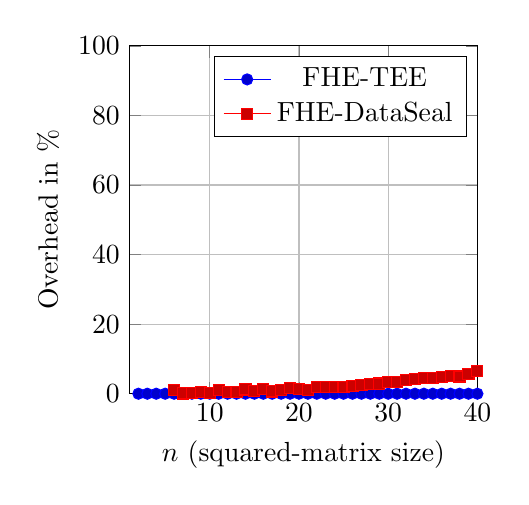
\begin{tikzpicture}
\begin{axis}[
    width=6cm, % Set the width of the plot to the text width of the subfigure
    height=6cm, % You can adjust the height as needed
    xlabel={$n$ (squared-matrix size)},
    ylabel={Overhead in \%},
    legend pos=north east,
    grid=both,
    xmin=1, xmax=40,
    ymin=0, ymax=100
]
\addplot table {
n   FHE-TEE
2	0
3	0
4	0
5	0
6	0
7	0
8	0
9	0
10	0
11	0
12	0
13	0
14	0
15	0
16	0
17	0
18	0
19	0
20	0
21	0
22	0
23	0
24	0
25	0
26	0
27	0
28	0
29	0
30	0
31	0
32	0
33	0
34	0
35	0
36	0
37	0
38	0
39	0
40	0

};
\addlegendentry{FHE-TEE}

\addplot table {
n   FHE-DataSeal
2	-0.4505441566
3	-0.1310558254
4	-0.1324889226
5	-0.3175549922
6	1.151792567
7	0.08521941232
8	0.2194850292
9	0.4011255793
10	0.2648147945
11	1.053044492
12	0.5583000423
13	0.5497135877
14	1.232912984
15	0.7900428124
16	1.291663451
17	0.6612845452
18	1.108591585
19	1.599185269
20	1.432558343
21	1.041985066
22	1.847595425
23	1.980300958
24	1.995841767
25	1.882570789
26	2.331824258
27	2.435739509
28	2.723598083
29	2.920616049
30	3.265554903
31	3.305986022
32	4.016227627
33	4.250366791
34	4.441436534
35	4.582011564
36	4.697349766
37	5.012025378
38	4.950407952
39	5.60946161
40	6.414157812
};
\addlegendentry{FHE-DataSeal}



\end{axis}
\end{tikzpicture}
